\documentclass[aspectratio=169]{beamer}
\usetheme{Boadilla}
%\usetheme{Warsaw}
%\setbeamercovered{transparent}
\beamertemplatetransparentcoveredhigh
\usepackage[portuges]{babel}
\usepackage[utf8]{inputenc}
\usepackage{lmodern}
\usepackage[T1]{fontenc}
\usepackage[portuguese, linesnumbered, vlined, titlenumbered, ruled]{algorithm2e}
\SetKwRepeat{Registro}{registro \{}{\}}%
\usepackage{hyperref} 

\usepackage{xcolor}
\definecolor{codegreen}{rgb}{0,0.6,0}
\definecolor{codegray}{rgb}{0.5,0.5,0.5}
\definecolor{codepurple}{rgb}{0.58,0,0.82}
\definecolor{backcolour}{rgb}{0.95,0.95,0.92}

\usepackage{listings}
\lstdefinestyle{CStyle}{
    language=C++,
    backgroundcolor=\color{backcolour},   
    commentstyle=\color{codegreen},
    keywordstyle=\color{magenta},
    numberstyle=\tiny\color{codegray},
    stringstyle=\color{codepurple},
    basicstyle=\ttfamily\footnotesize,
    breakatwhitespace=false,         
    breaklines=true,                 
    keepspaces=true,                 
    numbers=left,       
    numbersep=5pt,                  
    showspaces=false,                
    showstringspaces=false,
    showtabs=false,                  
    tabsize=2,
}

\newcommand{\eng}[1]{\textsl{#1}}
\newcommand{\cod}[1]{\texttt{#1}}

\title[Aula Prática Listas]{Listas Simplesmente Encadeadas\\
   Algoritmos e Estrutura de Dados}
\subtitle{Alocação Dinâmica}
\author[Frederico Santos de Oliveira]{prof. Frederico Santos de Oliveira}
\institute[UFMT]{Universidade Federal de Mato Grosso\\ Instituto de Engenharia}
\date{}

\AtBeginSection[]
{
	\begin{frame}
	\frametitle{Roteiro da Aula}
	\tableofcontents[currentsection]
\end{frame}
}

\begin{document}

%%%%%%%%%%%%%%%%%%%%%%%%%%%%%%%%%%%%%%%%%%%%%%%%%%%%%%%%%%%%%%%%%%%%%%%%%%%%%%%%%%%%%%%%%%%

\begin{frame}[plain]
  \titlepage
\end{frame}

%%%%%%%%%%%%%%%%%%%%%%%%%%%%%%%%%%%%%%%%%%%%%%%%%%%%%%%%%%%%%%%%%%%%%%%%%%%%%%%%%%%%%%%%%%%
%
%\begin{frame}
%  \frametitle{Agenda}
%  \tableofcontents
%\end{frame}


%%%%%%%%%%%%%%%%%%%%%%%%%%%%%%%%%%%%%%%%%%%%%%%%%%%%%%%%%%%%%%%%%%%%%%%%%%%%%%%%%%%%%%%%
\section{Introdução}
%%%%%%%%%%%%%%%%%%%%%%%%%%%%%%%%%%%%%%%%%%%%%%%%%%%%%%%%%%%%%%%%%%%%%%%%%%%%%%%%%%%%%%%%

\begin{frame}{Introdução}{Estrutura Nodo}
\begin{itemize}
 \item Assim como fizemos com a Pilha e a Fila, precisamos definir a estrutura de dados {\bf nodo}.
 \item O nodo é uma entidade elementar das estruturas de dados {\bf Pilha}, {\bf Fila} e {\bf Lista}. 
\end{itemize}
\end{frame}

%%%%%%%%%%%%%%%%%%%%%%%%%%%%%%%%%%%%%%%%%%%%%%%%%%%%%%%%%%%%%%%%%%%%%%%%%%%%%%%%%%%%%%%%

\begin{frame}{Introdução}{Estrutura Nodo}
Cada nodo armazena:
\begin{itemize}
 \item Um elemento.
  \begin{itemize}
  \item pode ser um inteiro, uma string, um vetor, um registro, não importa. 
  \item Aqui é denominado apenas {\bf item}.
  \end{itemize}  
 \item Uma ligação para o próximo nodo. 
 \begin{itemize}
 \item Em termos de implementação, trata-se de um ponteiro do tipo nodo, o qual denominaremos {\bf prox}.
 \end{itemize}
 \end{itemize}
\begin{figure}[!h]
  \centering
   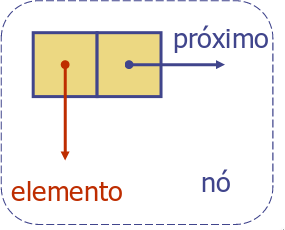
\includegraphics[width=100pt]{imagens/nodo.png}
  \label{fig_introducao}
\end{figure}
\end{frame}

%%%%%%%%%%%%%%%%%%%%%%%%%%%%%%%%%%%%%%%%%%%%%%%%%%%%%%%%%%%%%%%%%%%%%%%%%%%%%%%%%%%%%%%%

\begin{frame}[fragile]{Introdução}{Estrutura Nodo}
Primeiramente, vamos implementar o tipo de dados {\bf nodo}. Vamos analisar o pseudo-código apresentado nas aulas anteriores.
\end{frame}


%%%%%%%%%%%%%%%%%%%%%%%%%%%%%%%%%%%%%%%%%%%%%%%%%%%%%%%%%%%%%%%%%%%%%%%%%%%%%%%%%%%%%%%%

\begin{frame}[fragile]{Introdução}{Estrutura Nodo}
\begin{algorithm}[H]
\caption{Nodo} 
\label{Nodo}
\Inicio{
 \Registro{Nodo}{
    Inteiro: item; \\
    Ponteiro Nodo: prox; 
  }
}
\end{algorithm} 
\end{frame}

%%%%%%%%%%%%%%%%%%%%%%%%%%%%%%%%%%%%%%%%%%%%%%%%%%%%%%%%%%%%%%%%%%%%%%%%%%%%%%%%%%%%%%%%%%%%%%%%%%%%%

\begin{frame}[fragile]{Introdução}{Estrutura Nodo}
Na linguagem C, a implementação fica conforme o código a seguir:
\begin{lstlisting}[style=CStyle]
typedef struct nodo_t {
    int item;
    struct nodo_t *prox; 
} nodo;
\end{lstlisting}   
Vamos chamar o arquivo que contém esse código de \verb|nodo.h|.
\end{frame}


%%%%%%%%%%%%%%%%%%%%%%%%%%%%%%%%%%%%%%%%%%%%%%%%%%%%%%%%%%%%%%%%%%%%%%%%%%%%%%%%%%%%%%%%
\section{Exercício 1}
%%%%%%%%%%%%%%%%%%%%%%%%%%%%%%%%%%%%%%%%%%%%%%%%%%%%%%%%%%%%%%%%%%%%%%%%%%%%%%%%%%%%%%%%

\begin{frame}{Exercício 1}{Lista Simples}
Neste exercício, vamos implementar a estrutura de dados {\bf Lista Simplesmente Encadeada}:
\begin{itemize}
 \item Nessa estrutura existem dois ponteiros:
 \begin{itemize}
    \item um aponta para o {\bf primeiro} nodo da Lista.
    \item o outro que aponta para o {\bf último} nodo da Lista.
 \end{itemize}
 \item Diferentemente da Pilha e da Fila, \underline{não existe} o nodo {\bf cabeça}.
 \item Quando a Lista está vazia, os ponteiros primeiro e último apontam para NULL.
\end{itemize}
\end{frame}

%%%%%%%%%%%%%%%%%%%%%%%%%%%%%%%%%%%%%%%%%%%%%%%%%%%%%%%%%%%%%%%%%%%%%%%%%%%%%%%%%%%%%%%%

\begin{frame}{Exercício 1}{Lista Simples}
\begin{algorithm}[H]
\caption{Lista} 
\label{Lista}
\Inicio{
 \Registro{Lista}{
    Ponteiro Nodo: primeiro, último; 
  }
}
\end{algorithm} 
\end{frame}

%%%%%%%%%%%%%%%%%%%%%%%%%%%%%%%%%%%%%%%%%%%%%%%%%%%%%%%%%%%%%%%%%%%%%%%%%%%%%%%%%%%%%%%%%%%%%%%%%%%%%

\begin{frame}[fragile]{Exercício 1}{Lista Simples}
Na linguagem C, a implementação fica conforme o código a seguir:
\begin{lstlisting}[style=CStyle]
#include "nodo.h"
typedef struct {
  nodo *primeiro;
  nodo *ultimo;
} lista;
\end{lstlisting}  
Vamos chamar o arquivo que contém esse código de \verb|lista.h|.
\end{frame}

%%%%%%%%%%%%%%%%%%%%%%%%%%%%%%%%%%%%%%%%%%%%%%%%%%%%%%%%%%%%%%%%%%%%%%%%%%%%%%%%%%%%%%%%%%%%%%%%%%%%%

\begin{frame}[fragile]{Exercício 1}{Lista Simples}
A seguir, vamos implementar a função CriarListaVazia($L$).
\end{frame}

%%%%%%%%%%%%%%%%%%%%%%%%%%%%%%%%%%%%%%%%%%%%%%%%%%%%%%%%%%%%%%%%%%%%%%%%%%%%%%%%%%%%%%%%%%%%%%%%%%%%%

\begin{frame}[fragile]{Exercício 2}{Lista Simples}
Vamos adicionar o protótipo dessa função no arquivo \verb|lista.h|.
\begin{lstlisting}[style=CStyle]
void criarListaVazia(lista *l);
\end{lstlisting}  
Agora, vamos implementar essa função. 
\end{frame}


%%%%%%%%%%%%%%%%%%%%%%%%%%%%%%%%%%%%%%%%%%%%%%%%%%%%%%%%%%%%%%%%%%%%%%%%%%%%%%%%%%%%%%%%%%%%%%%%%%%%%

\begin{frame}[fragile]{Exercício 1}{Lista Simples}
\begin{itemize}
\item Primeiramente, vamos criar um arquivo chamado \verb|lista.c| que deve conter a implementação dessas funções.
\item Para evitar que o compilador não encontre determinada função, vamos incluir o protótipo das funções, inserindo a linha de código a seguir no início do arquivo \verb|lista.c|:
\begin{lstlisting}[style=CStyle]
#include "lista.h"
\end{lstlisting}  
\item A seguir, vamos implementar a função CriarListaVazia($L$), que recebe uma lista L e aponta devidamente os ponteiros \verb|primeiro| e \verb|ultimo|. 
\end{itemize} 
\end{frame}

%%%%%%%%%%%%%%%%%%%%%%%%%%%%%%%%%%%%%%%%%%%%%%%%%%%%%%%%%%%%%%%%%%%%%%%%%%%%%%%%%%%%%%%%%%%%%%%%%%%%%

\begin{frame}[fragile]{Exercício 1}{Lista Simples}
% \scalebox{0.5}{
\begin{algorithm}[H]
\caption{CriarListaVazia} 
\label{CriarListaVazia}
\Entrada{Lista L.}
\Inicio{
  L.primeiro $\leftarrow$ NULL \\
  L.último $\leftarrow$ NULL \\
}
\end{algorithm}
\end{frame}

%%%%%%%%%%%%%%%%%%%%%%%%%%%%%%%%%%%%%%%%%%%%%%%%%%%%%%%%%%%%%%%%%%%%%%%%%%%%%%%%%%%%%%%%%%%%%%%%%%%%%

\begin{frame}[fragile]{Exercício 1}{Lista Simples}
Na linguagem C, a implementação fica conforme o código a seguir:
\begin{lstlisting}[style=CStyle]
void criarListaVazia(lista *l) {
    l->primeiro = NULL ;
    l->ultimo = NULL ;
}
\end{lstlisting}  
\end{frame}


%%%%%%%%%%%%%%%%%%%%%%%%%%%%%%%%%%%%%%%%%%%%%%%%%%%%%%%%%%%%%%%%%%%%%%%%%%%%%%%%%%%%%%%%%%%%%%%%%%%%%

\begin{frame}[fragile]{Exercício 1}{Lista Simples}
A seguir, vamos implementar a função ListaVazia($L$), que verifica se uma lista está vazia.
\end{frame}

%%%%%%%%%%%%%%%%%%%%%%%%%%%%%%%%%%%%%%%%%%%%%%%%%%%%%%%%%%%%%%%%%%%%%%%%%%%%%%%%%%%%%%%%%%%%%%%%%%%%%

\begin{frame}[fragile]{Exercício 1}{Lista Simples}
% \scalebox{0.5}{
\begin{algorithm}[H]
\caption{ListaVazia} 
\label{ListaVazia}
\Entrada{Lista L.}
\Saida{Booleano (V ou F) indicando se L está vazia.}
\Inicio{
  \Se {(L.primeiro = NULL)} {
    \Retorna Verdadeiro
  }
  \Senao {
    \Retorna Falso
  }
}
\end{algorithm}
\end{frame}

%%%%%%%%%%%%%%%%%%%%%%%%%%%%%%%%%%%%%%%%%%%%%%%%%%%%%%%%%%%%%%%%%%%%%%%%%%%%%%%%%%%%%%%%%%%%%%%%%%%%%

\begin{frame}[fragile]{Exercício 1}{Lista Simples}
Na linguagem C, a implementação fica conforme o código a seguir:
\begin{lstlisting}[style=CStyle]
int listaVazia(lista * l ) {
    return l->primeiro == NULL ;
}
\end{lstlisting}  
\end{frame}

%%%%%%%%%%%%%%%%%%%%%%%%%%%%%%%%%%%%%%%%%%%%%%%%%%%%%%%%%%%%%%%%%%%%%%%%%%%%%%%%%%%%%%%%%%%%%%%%%%%%%

\begin{frame}[fragile]{Exercício 1}{Lista Simples}
A seguir, vamos implementar a função InserirInicio($L$, $x$), que insere o elemento $x$ no início de uma lista.
\end{frame}

%%%%%%%%%%%%%%%%%%%%%%%%%%%%%%%%%%%%%%%%%%%%%%%%%%%%%%%%%%%%%%%%%%%%%%%%%%%%%%%%%%%%%%%%%%%%%%%%%%%%%

\begin{frame}[fragile]{Exercício 1}{Lista Simples}
\begin{algorithm}[H]
\caption{InserirInício} 
\label{ListaSimplesInserirInicio}
\Entrada{Lista L, item $x$.}
\Inicio{
  novo $\leftarrow ALOCA\_NODO()$ \\
  novo.item $\leftarrow$ x \\
  novo.prox $\leftarrow$ L.primeiro \\
  L.primeiro $\leftarrow$ novo \\
  \CommentSty{// Verifica se a lista está vazia.} \\
  \Se {(L.último = NULL)} {
    L.último $\leftarrow$ L.primeiro \\
  }
}
\end{algorithm}
\end{frame}

%%%%%%%%%%%%%%%%%%%%%%%%%%%%%%%%%%%%%%%%%%%%%%%%%%%%%%%%%%%%%%%%%%%%%%%%%%%%%%%%%%%%%%%%%%%%%%%%%%%%%

\begin{frame}[fragile]{Exercício 1}{Lista Simples}
Na linguagem C, a implementação fica conforme o código a seguir:
\begin{lstlisting}[style=CStyle]
void inserirInicio(lista *l, int x ) {
    nodo *novo = malloc(sizeof(nodo));
    novo->item = x;
    novo->prox = l->primeiro;
    if (l->primeiro == NULL) 
        l->ultimo = novo ;
    l->primeiro = novo ;
}
\end{lstlisting}  
\end{frame}

%%%%%%%%%%%%%%%%%%%%%%%%%%%%%%%%%%%%%%%%%%%%%%%%%%%%%%%%%%%%%%%%%%%%%%%%%%%%%%%%%%%%%%%%%%%%%%%%%%%%%

\begin{frame}[fragile]{Exercício 1}{Lista Simples}
A seguir, vamos implementar a função InserirFinal($L$, $x$), que insere o elemento $x$ no final de uma lista.
\end{frame}

%%%%%%%%%%%%%%%%%%%%%%%%%%%%%%%%%%%%%%%%%%%%%%%%%%%%%%%%%%%%%%%%%%%%%%%%%%%%%%%%%%%%%%%%%%%%%%%%%%%%%

\begin{frame}[fragile]{Exercício 1}{Lista Simples}
% \scalebox{0.5}{
\begin{algorithm}[H]
\caption{InserirFinal} 
\label{ListaSimplesInserirFinal}
\Entrada{Lista L, item $x$.}
\Inicio{
  novo $\leftarrow ALOCA\_NODO()$ \\
  novo.item $\leftarrow$ x \\
  novo.prox $\leftarrow$ NULL \\
  \CommentSty{// Verifica se a lista está vazia.} \\
  \Se {(L.primeiro = NULL)} {
    L.primeiro $\leftarrow$ novo \\
    L.último $\leftarrow$ L.primeiro \\
  }
  \Senao {
    L.último.prox $\leftarrow$ novo \\
    L.último $\leftarrow$ novo \\
  }
}
\end{algorithm}
% }  
\end{frame}

%%%%%%%%%%%%%%%%%%%%%%%%%%%%%%%%%%%%%%%%%%%%%%%%%%%%%%%%%%%%%%%%%%%%%%%%%%%%%%%%%%%%%%%%%%%%%%%%%%%%%

\begin{frame}[fragile]{Exercício 1}{Lista Simples}
Na linguagem C, a implementação fica conforme o código a seguir:
\begin{lstlisting}[style=CStyle]
void inserirFinal (lista *l, int x ) {
    nodo *novo = malloc(sizeof(nodo)) ;
    novo->item = x ;
    novo->prox = NULL ;
    if (l->primeiro == NULL ) 
        l->primeiro = novo ;
    else 
        l->ultimo->prox = novo ;    
    l->ultimo = novo ;
}
\end{lstlisting}  
\end{frame}

%%%%%%%%%%%%%%%%%%%%%%%%%%%%%%%%%%%%%%%%%%%%%%%%%%%%%%%%%%%%%%%%%%%%%%%%%%%%%%%%%%%%%%%%%%%%%%%%%%%%%

\begin{frame}[fragile]{Exercício 1}{Lista Simples}
A seguir, vamos implementar a função BuscarPosicao($L$, $p$), que retorna um ponteiro para o nodo na posição $p$ de uma lista.
\end{frame}

%%%%%%%%%%%%%%%%%%%%%%%%%%%%%%%%%%%%%%%%%%%%%%%%%%%%%%%%%%%%%%%%%%%%%%%%%%%%%%%%%%%%%%%%%%%%%%%%%%%%%

\begin{frame}[fragile]{Exercício 1}{Lista Simples}
% \scalebox{0.5}{
\begin{algorithm}[H]
\caption{BuscarPosicao} 
\label{ListaSimplesBuscar}
\Entrada{Lista L, item $p$.}
\Saida{Nodo na posição $p$ ou NULL caso não encontrado.}
\Inicio{
  aux $\leftarrow$ L.primeiro \\
  c $\leftarrow$ 1 \\
  \Enqto {(aux $\neq$ NULL) AND (c $<$ p) } {
      aux $\leftarrow$ aux.prox \\
      c $\leftarrow$ c + 1 \\
  }
  \Retorna aux
}
\end{algorithm}
% }  
\end{frame}

%%%%%%%%%%%%%%%%%%%%%%%%%%%%%%%%%%%%%%%%%%%%%%%%%%%%%%%%%%%%%%%%%%%%%%%%%%%%%%%%%%%%%%%%%%%%%%%%%%%%%

\begin{frame}[fragile]{Exercício 1}{Lista Simples}
Na linguagem C, a implementação fica conforme o código a seguir:
%\begin{lstlisting}[style=CStyle,basicstyle=\tiny]]
\begin{lstlisting}[style=CStyle]]
nodo *buscarPosicao(lista *l, int p ) {
    nodo *aux = l->primeiro;
    int c = 1;
    while ( aux != NULL && c < p ) {
        aux = aux->prox;
        c ++;
    }
    return aux;
}
\end{lstlisting}  
\end{frame}

%%%%%%%%%%%%%%%%%%%%%%%%%%%%%%%%%%%%%%%%%%%%%%%%%%%%%%%%%%%%%%%%%%%%%%%%%%%%%%%%%%%%%%%%%%%%%%%%%%%%%

\begin{frame}[fragile]{Exercício 1}{Lista Simples}
A seguir, vamos implementar a função inserirPosicao($L$, $x$, $p$), que insere um elemento $x$ na posição $p$ de uma lista.
\end{frame}

%%%%%%%%%%%%%%%%%%%%%%%%%%%%%%%%%%%%%%%%%%%%%%%%%%%%%%%%%%%%%%%%%%%%%%%%%%%%%%%%%%%%%%%%%%%%%%%%%%%%%

\begin{frame}[fragile]{Exercício 1}{Lista Simples}
\scalebox{0.6} {
\begin{algorithm}[H]
\caption{InserirPosição} 
\label{ListaSimplesInserirPosicao}
\Entrada{Lista L, item $x$, posição $p$.}
\Inicio{
  \CommentSty{// Verifica se o nodo deve ser inserido no início. }\\
  \Se {($p = 1$)} {
    ListaInserirInício(L, x) \\
  }
  \Senao {
    novo $\leftarrow ALOCA\_NODO()$ \\
    novo.item $\leftarrow$ x \\  
    \CommentSty{// Busca o nodo na posição anterior a $p$.}\\
    anterior $\leftarrow$ BuscarPosição(L,$p-1$) \\
    \CommentSty{// Insere o novo nodo entre os nodos} \\
    \CommentSty{// anterior e posterior.}\\
    posterior $\leftarrow$ anterior.prox \\
    anterior.prox $\leftarrow$ novo \\  
    novo.prox $\leftarrow$ posterior \\
    \CommentSty{// Verifica se o nodo na posição $p-1$ é o último,}\\
    \CommentSty{// ou seja, seu posterior é NULL.} \\
    \Se {(posterior = NULL)} {
      L.último $\leftarrow$ novo \\
    }   
  }
}
\end{algorithm}
}% scalebox  
\end{frame}

%%%%%%%%%%%%%%%%%%%%%%%%%%%%%%%%%%%%%%%%%%%%%%%%%%%%%%%%%%%%%%%%%%%%%%%%%%%%%%%%%%%%%%%%%%%%%%%%%%%%%

\begin{frame}[fragile]{Exercício 1}{Lista Simples}
Na linguagem C, a implementação fica conforme o código a seguir:
%\begin{lstlisting}[style=CStyle,basicstyle=\tiny]]
\begin{lstlisting}[style=CStyle]]
void inserirPosicao (lista *l, int x, int p ) {
    if (p ==1)
        inserirInicio(l, x);
    else {
        nodo *anterior = l->primeiro, *posterior;
        nodo *novo = malloc(sizeof(nodo));
        novo->item = x ;
        anterior = buscarPosicao(l ,p -1);
        posterior = anterior->prox;
        anterior->prox = novo;
        novo-> prox = posterior;
        if (posterior == NULL )
            l->ultimo = novo;
    }
}
\end{lstlisting}  
\end{frame}

%%%%%%%%%%%%%%%%%%%%%%%%%%%%%%%%%%%%%%%%%%%%%%%%%%%%%%%%%%%%%%%%%%%%%%%%%%%%%%%%%%%%%%%%%%%%%%%%%%%%%

\begin{frame}[fragile]{Exercício 1}{Lista Simples}
A seguir, vamos implementar a função RemoverInicio($L$), que remove um elemento que se encontra no início de uma lista.
\end{frame}

%%%%%%%%%%%%%%%%%%%%%%%%%%%%%%%%%%%%%%%%%%%%%%%%%%%%%%%%%%%%%%%%%%%%%%%%%%%%%%%%%%%%%%%%%%%%%%%%%%%%%

\begin{frame}[fragile]{Exercício 1}{Lista Simples}
\scalebox{0.8}{
\begin{algorithm}[H]
\caption{RemoverInício} 
\label{ListaSimplesRemoverInicio}
\Entrada{Lista L, item $x$.}
\Inicio{
  \CommentSty{// Verifica se a lista está vazia.} \\
  \Se {(ListaVazia(L))} {
      Imprima "Erro {\it underflow}: lista vazia" \\ 
  }
  \Senao {
    aux $\leftarrow$ L.primeiro \\    
    x $\leftarrow$ aux.item \\
    L.primeiro $\leftarrow$ L.primeiro.prox \\
    \CommentSty{// Verifica se a lista possui apenas um nodo.} \\
    \Se {(L.primeiro = NULL)} {
      \CommentSty{// Primeiro e Último apontam para NULL.} \\
      L.último $\leftarrow$ NULL \\
    }
    aux.prox $\leftarrow$ NULL \\
    DESALOCA\_NODO(aux) \\
    \Retorna x
  }
}
\end{algorithm}
} 
\end{frame}

%%%%%%%%%%%%%%%%%%%%%%%%%%%%%%%%%%%%%%%%%%%%%%%%%%%%%%%%%%%%%%%%%%%%%%%%%%%%%%%%%%%%%%%%%%%%%%%%%%%%%

\begin{frame}[fragile]{Exercício 1}{Lista Simples}
%\begin{lstlisting}[style=CStyle,basicstyle=\tiny]]
\begin{lstlisting}[style=CStyle]
int removerInicio(lista * l) {
    nodo * aux;
    int x = -1;
    if (listaVazia(l) )
        printf("Lista Vazia\n");
    else {
        aux = l->primeiro;
        x = aux->item;
        l->primeiro = l->primeiro->prox;
        if (l->primeiro == NULL)
           l->ultimo = NULL;
        aux->prox = NULL;
        free(aux);
    }
    return x;
}
\end{lstlisting}  
\end{frame}

%%%%%%%%%%%%%%%%%%%%%%%%%%%%%%%%%%%%%%%%%%%%%%%%%%%%%%%%%%%%%%%%%%%%%%%%%%%%%%%%%%%%%%%%%%%%%%%%%%%%%

\begin{frame}[fragile]{Exercício 1}{Lista Simples}
A seguir, vamos implementar a função RemoverFinal($L$), que remove um elemento que se encontra no final de uma lista.
\end{frame}

%%%%%%%%%%%%%%%%%%%%%%%%%%%%%%%%%%%%%%%%%%%%%%%%%%%%%%%%%%%%%%%%%%%%%%%%%%%%%%%%%%%%%%%%%%%%%%%%%%%%%

\begin{frame}[fragile]{Exercício 1}{Lista Simples}
\scalebox{0.5}{
\begin{algorithm}[H]
\caption{RemoverFinal} 
\label{ListaSimplesRemoverFinal}
\Entrada{Lista L}
\Saida{Item removido}
\Inicio{
  \CommentSty{// Verifica se a lista está vazia.} \\
  \Se {(ListaVazia(L))} {
      Imprima "Erro {\it underflow}: lista vazia" \\ 
  }  
  \Senao {
    \CommentSty{// Verifica se a lista possui um único elemento.} \\  
    \Se{(L.primeiro = L.último) AND (NOT(ListaVazia(L)))} {
	aux $\leftarrow$ L.primeiro\\
	L.primeiro $\leftarrow$ NULL \\
	L.último $\leftarrow$ NULL \\
    }
    \CommentSty{// Caso contrário, a lista possui }\\
    \CommentSty{// pelo menos dois elementos.} \\  
    \Senao {
     \CommentSty{// Busca o penúltimo elemento.} \\  
      anterior $\leftarrow$ L.primeiro \\    
      \Enqto{(anterior.prox $\neq$ L.último)} {
		anterior $\leftarrow$ anterior.prox \\
      }
      aux $\leftarrow$ L.último \\
      anterior.prox $\leftarrow$ NULL \\
      L.último $\leftarrow$ anterior \\
    }
    x $\leftarrow$  aux.item \\
    aux.prox $\leftarrow$ NULL \\
    DESALOCA\_NODO(aux) \\  
    \Retorna x
  }
}
\end{algorithm}
}  
\end{frame}

%%%%%%%%%%%%%%%%%%%%%%%%%%%%%%%%%%%%%%%%%%%%%%%%%%%%%%%%%%%%%%%%%%%%%%%%%%%%%%%%%%%%%%%%%%%%%%%%%%%%%

\begin{frame}[fragile]{Exercício 1}{Lista Simples}
\begin{lstlisting}[style=CStyle,basicstyle=\tiny]]
int removerFinal(lista *l) {
    int x = -1;
    nodo *aux, *anterior;
    if (listaVazia(l))
        printf("Lista Vazia\n") ;
    else if (l->primeiro == l->ultimo) {
        aux = l->primeiro;
        l->primeiro = NULL;
        l->ultimo = NULL;
    }
    else {
        anterior = l->primeiro;
        while (anterior->prox != l->ultimo)
            anterior = anterior->prox;
        aux = l->ultimo;
        anterior->prox = NULL;
        l->ultimo = anterior;
    }
    x = aux->item ;
    aux->prox = NULL ;
    free(aux) ;
    return x ;
}
\end{lstlisting}  
\end{frame}

%%%%%%%%%%%%%%%%%%%%%%%%%%%%%%%%%%%%%%%%%%%%%%%%%%%%%%%%%%%%%%%%%%%%%%%%%%%%%%%%%%%%%%%%%%%%%%%%%%%%%

\begin{frame}[fragile]{Exercício 1}{Lista Simples}
A seguir, vamos implementar a função removerPosicao($L$, $p$), que remove um elemento que se encontra na posição $p$ de uma lista.
\end{frame}

%%%%%%%%%%%%%%%%%%%%%%%%%%%%%%%%%%%%%%%%%%%%%%%%%%%%%%%%%%%%%%%%%%%%%%%%%%%%%%%%%%%%%%%%%%%%%%%%%%%%%

\begin{frame}[fragile]{Exercício 1}{Lista Simples}
\scalebox{0.56} {
\begin{algorithm}[H]
\caption{RemoverPosição} 
\label{ListaSimplesRemoverPosicao}
\Entrada{Lista L, posição $p$}
\Saida{Item removido}
\Inicio{
  \CommentSty{// Verifica se a lista está vazia.} \\
  \Se {(ListaVazia(L))} {
      Imprima "Erro {\it underflow}: lista vazia" \\ 
  }
  \Senao {
    \CommentSty{// Verifica se o nodo a ser removido é o primeiro.}\\
    \Se {(p = 1)} {
      \Retorna RemoverInicio(L) \\
    }
    \Senao {
      \CommentSty{// Busca o nodo na posição anterior a $p$.}\\
      anterior $\leftarrow$ ListaBuscarPosição(L,$p-1$) \\
      \CommentSty{// Remove o nodo na posição $p$, apontado por aux.}\\
      aux $\leftarrow$ anterior.prox \\
      posterior $\leftarrow$ aux.prox \\  
      anterior.prox $\leftarrow$ posterior \\
      \CommentSty{// Verifica se o nodo a ser removido é o último.}\\
      \Se {(aux = L.último)}  {
	L.último $\leftarrow$ anterior \\
      }   
      $x \leftarrow$ aux.item \\
      aux.prox $\leftarrow$ NULL \\
      DESALOCA\_NODO(aux) \\
      \Retorna $x$
    }
  }
}
\end{algorithm}
}% scalebox  
\end{frame}

%%%%%%%%%%%%%%%%%%%%%%%%%%%%%%%%%%%%%%%%%%%%%%%%%%%%%%%%%%%%%%%%%%%%%%%%%%%%%%%%%%%%%%%%%%%%%%%%%%%%%

\begin{frame}[fragile]{Exercício 1}{Lista Simples}
\begin{lstlisting}[style=CStyle,basicstyle=\tiny]]
int removerPosicao(lista *l, int p) {
    int x = -1;
    nodo *anterior, *posterior, *aux;
    if (p==1)
        x = removerInicio(l);
    else {    
        anterior = buscarPosicao(l,p-1);
        aux = anterior->prox;
        posterior = aux->prox;
        anterior->prox = posterior;
        if (aux == l->ultimo)
            l->ultimo = anterior;
        x = aux->item;
        aux->prox = NULL;
        free(aux);
    }
    return x;    
}		
\end{lstlisting}  
\end{frame}

%%%%%%%%%%%%%%%%%%%%%%%%%%%%%%%%%%%%%%%%%%%%%%%%%%%%%%%%%%%%%%%%%%%%%%%%%%%%%%%%%%%%%%%%%%%%%%%%%%%%%

\begin{frame}[fragile]{Exercício 1}{Lista Simples}
\begin{itemize}
\item Ainda falta uma função: aquela que apaga todos os nodos de uma lista.
\item Vamos implementá-la a seguir.
\end{itemize}
\end{frame}


%%%%%%%%%%%%%%%%%%%%%%%%%%%%%%%%%%%%%%%%%%%%%%%%%%%%%%%%%%%%%%%%%%%%%%%%%%%%%%%%%%%%%%%%%%%%%%%%%%%%%

\begin{frame}[fragile]{Exercício 1}{Lista Simples}
% \scalebox{0.5}{
\begin{algorithm}[H]
\caption{ApagarLista} 
\label{ApagarLista}
\Entrada{Lista L.}
\Inicio{
  aux $\leftarrow$ L.primeiro \\
  \Enqto {(L.primeiro $\neq$ NULL)} {
    L.primeiro $\leftarrow$ L.primeiro.prox \\
    DESALOCA\_NODO(aux) \\
    aux = L.primeiro 
  }
}
\end{algorithm}
% }  
\end{frame}

%%%%%%%%%%%%%%%%%%%%%%%%%%%%%%%%%%%%%%%%%%%%%%%%%%%%%%%%%%%%%%%%%%%%%%%%%%%%%%%%%%%%%%%%%%%%%%%%%%%%%

\begin{frame}[fragile]{Exercício 1}{Lista Simples}
Na linguagem C, a implementação fica conforme o código a seguir:
\begin{lstlisting}[style=CStyle]
void apagarLista(lista *l) {
  nodo *aux = l->primeiro;
  while (aux != NULL) {
    l->primeiro = l->primeiro->prox;
    free(aux);   
    aux = l->primeiro;
  }
}
\end{lstlisting}  
\end{frame}

%%%%%%%%%%%%%%%%%%%%%%%%%%%%%%%%%%%%%%%%%%%%%%%%%%%%%%%%%%%%%%%%%%%%%%%%%%%%%%%%%%%%%%%%%%%%%%%%%%%%%

\begin{frame}[fragile]{Exercício 1}{Lista Simples}
Vamos implementar a função que imprime os valores de uma lista.
\end{frame}


%%%%%%%%%%%%%%%%%%%%%%%%%%%%%%%%%%%%%%%%%%%%%%%%%%%%%%%%%%%%%%%%%%%%%%%%%%%%%%%%%%%%%%%%%%%%%%%%%%%%%

\begin{frame}[fragile]{Exercício 1}{Lista Simples}
% \scalebox{0.5}{
\begin{algorithm}[H]
\caption{ImprimirLista} 
\label{imprimirLista}
\Entrada{Lista L.}
\Inicio{
  aux $\leftarrow$ L.primeiro \\
  \Enqto {(aux $\neq$ NULL)} {
  	Imprima(aux.item) \\
    aux = aux.prox \\ 
  }
}
\end{algorithm}
% }  
\end{frame}

%%%%%%%%%%%%%%%%%%%%%%%%%%%%%%%%%%%%%%%%%%%%%%%%%%%%%%%%%%%%%%%%%%%%%%%%%%%%%%%%%%%%%%%%%%%%%%%%%%%%%

\begin{frame}[fragile]{Exercício 1}{Lista Simples}
Na linguagem C, a implementação fica conforme o código a seguir:
\begin{lstlisting}[style=CStyle]
void imprimirLista(lista *l) {
  nodo *aux = l->primeiro;
  while (aux != NULL) {
    printf("%d ", aux->item);
    aux = aux->prox;
  }
  printf("\n");
}
\end{lstlisting}  
\end{frame}

%%%%%%%%%%%%%%%%%%%%%%%%%%%%%%%%%%%%%%%%%%%%%%%%%%%%%%%%%%%%%%%%%%%%%%%%%%%%%%%%%%%%%%%%%%%%%%%%%%%%%

\begin{frame}[fragile]{Exercício 1}{Lista Simples}
Após implementar essas funções, faça o teste, inserindo e removendo alguns valores.
\end{frame}

%%%%%%%%%%%%%%%%%%%%%%%%%%%%%%%%%%%%%%%%%%%%%%%%%%%%%%%%%%%%%%%%%%%%%%%%%%%%%%%%%%%%%%%%%%%%%%%%%%%%%

\begin{frame}[fragile]{Exercício 1}{Lista Simples}
Em um arquivo chamado \verb|executa_lista.c|, insira  o código a seguir:
\begin{lstlisting}[style=CStyle]
#include "lista.h"
int main() {
  int i;
  lista *l = malloc(sizeof(lista));
  criarListaVazia(l);
  for (i=0; i<10; i++) {
    inserirInicio(l,i);
    printf("Inseriu Inicio %d\n",i);    
  }
  for (i=-1;i>-3;i--) {
    inserirFinal(l,i);
    printf("Inseriu final %d\n",i);
  }  
  printf("Inseriu %d na posicao 4\n",10);
  inserirPosicao(l,10,4);
  imprimirLista(l);
  /** Continua no proximo slide **/
}
\end{lstlisting}  
\end{frame}

%%%%%%%%%%%%%%%%%%%%%%%%%%%%%%%%%%%%%%%%%%%%%%%%%%%%%%%%%%%%%%%%%%%%%%%%%%%%%%%%%%%%%%%%%%%%%%%%%%%%%

\begin{frame}[fragile]{Exercício 1}{Lista Simples}
\begin{lstlisting}[style=CStyle]
#include "lista.h"
int main() {
  /** Codigo anterior **/
  i = removerInicio(l);
  printf("Removeu Inicio %d\n",i);
  imprimirLista(l);
  i = removerFinal(l);
  printf("Removeu Final %d\n",i);
  imprimirLista(l);
  i = removerInicio(l);
  printf("Removeu Inicio %d\n",i);
  imprimirLista(l);
  i = removerPosicao(l,7);
  printf("Removeu %d na posicao %d\n",i,7);
  apagarLista(l);
  printf("Apagou a lista\n");
  free(l);
}
\end{lstlisting}  
\end{frame}

%%%%%%%%%%%%%%%%%%%%%%%%%%%%%%%%%%%%%%%%%%%%%%%%%%%%%%%%%%%%%%%%%%%%%%%%%%%%%%%%%%%%%%%%%%%

\begin{frame}[plain]
  \titlepage
\end{frame}

\end{document}
